\chapter{The Compact Muon Solenoid experiment \label{chap:CMS}}

The Compact Muon Solenoid (CMS)~\cite{Chatrchyan:2008aa,Bayatian:922757,Ball:2007zza,CMS_website} is
one of the two general purpose detectors
at the LHC. It is
located on the far-end of the LHC ring, at interaction point 5 (P5) in Cessy, France. 
Like most collider experiments, CMS has a cylindrical shape, consisting of a barrel region and two
so-called endcaps at either end of the barrel. The various subdetector systems are layered around
the collision point. The central feature of the CMS detector is the superconducting solenoid with
high magnetic field to achieve good momentum resolution. The muon systems are installed in between
the return yoke layers. The silicon tracker, lead-tungstate crystal electromagnetic calorimeter
(ECAL), and brass scintillator hadron calorimeter (HCAL) are contained within the bore of the magnet
coil. 
The CMS detector has a length of 21\meter, a diameter of 15\meter and a total weight of $14\,000$
tonnes. 
Figure~\ref{fig:cms_overview} shows an overview of the detector and its different
subsystems. It is important to note that different kinds of particles interact differently with the
various subdetectors, as illustrated in Fig.~\ref{fig:cms_slice}. This design allows the
reconstruction software to distinguish between electrons, muons, photons, charged and neutral
hadrons. 
A more extensive discussion on each subsystem will be given in the
following sections. 

\begin{figure}[htpb]
  \centering
  \includegraphics[width=0.9\textwidth]{figures/cms/CMS_overview_labelled}
  \caption{Overview of the CMS detector. The different subsystems are indicated on the figure, as
well as a person to serve as reference scale. Figure taken from Ref. \cite{CMS_overview_labelled}.
  \label{fig:cms_overview}}
\end{figure}

\begin{figure}[htpb]
  \centering
  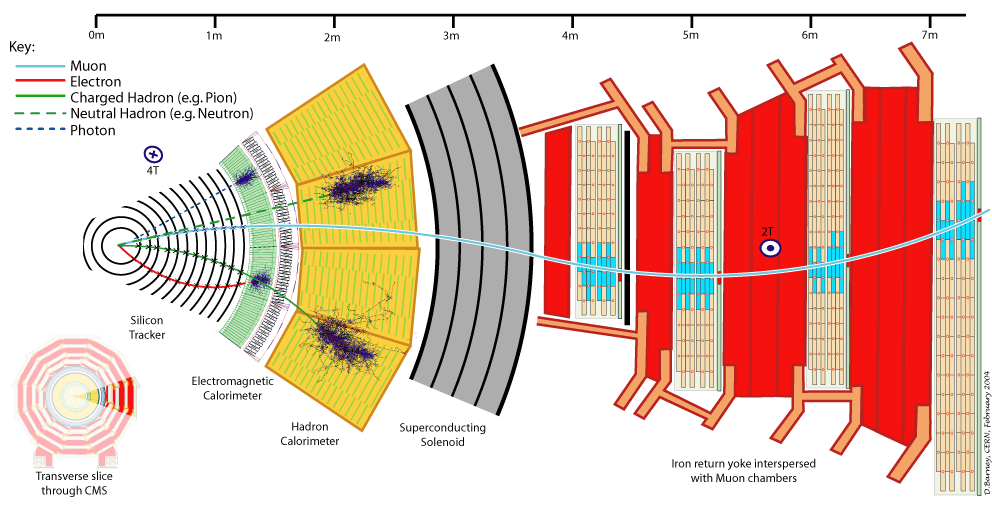
\includegraphics[width=0.9\textwidth]{figures/cms/CMS_Slice}
  \caption{Detailed view of a CMS detector slice, showing the interactions of different kinds of
particles with the various subsystems. Muons leave hits in the tracker and the muon stations,
before leaving the detector. Electrons leave hits in the tracker, and then deposit their
energy in the ECAL. Photons can be identified as an energy deposit in the ECAL without a
corresponding track. Charged and neutral hadrons both deposit their energy in the HCAL, with
matching tracker hits for charged hadrons only. 
Figure taken from Ref.~\cite{CMS_slice}.
  \label{fig:cms_slice}}
\end{figure}

%%%%%%%%%%%%%%%%%%%%%%%%%%%%%%%%%%%%%%%%%%%%%%%%%%%%%%%%%%%%%%%%%%%%%%%%%%%%%%%%%%%%%%%%%%%%%%%%%%%%
\section{Coordinate system and basic variables \label{sec:cms_coordinates}}

The CMS coordinate system takes the nominal collision point as the origin, with the $y$-axis
pointing vertically upward, and the $x$-axis pointing radially inward towards the centre of the
LHC. The coordinate system is right-handed, such that the $z$-axis points along the beam direction
toward the Jura mountains as seen from P5. 
The azimuthal angle $\phi$ is measured from the $x$-axis in the ($x,y$) plane. The polar angle
$\theta$ is measured from the $z$-axis. 
Pseudorapidity $\eta$ is defined as 
\begin{equation}
 \eta = - \ln \left[ \tan(\theta/2) \right],  
\end{equation}
and is usually used instead of the
polar angle because of the property that differences in pseudorapidity are
Lorentz-invariant. This is especially useful for hadron colliders where the boost in the $z$
direction is unknown, and varies for each collision. A Lorentz-invariant angular separation between
two particles is defined as 
\begin{equation}
\Delta R = \sqrt{(\Delta\eta)^2 + (\Delta\phi)^2}.
\end{equation}
The momentum and energy measured transverse to the beam direction, denoted by $\pt$ and $\ET$,
respectively, are computed from the $x$ and $y$ components.
The imbalance of energy measured in the transverse plane is denoted by \ETm, and indicates
undetected particles, or energy mismeasurements.
 

% 1.3.1 Summary of detector requirements
% The detector requirements for CMS to meet the goals of the LHC physics programme can be
% summarized as follows:
% • Good muon identification and momentum resolution over a wide range of momenta
% in the region |η| < 2.5, good dimuon mass resolution (≈ 1% at 100 GeV/c2),
% and the ability to determine unambiguously the charge of muons with p < 1 TeV/c.
% • Good charged particle momentum resolution and reconstruction efficiency in the
% inner tracker. Efficient triggering and offline tagging of τ ’s and b-jets, requiring1.4.
% Experimental challenge 7
% pixel detectors close to the interaction region.
% • Good electromagnetic energy resolution, good diphoton and dielectron mass resolution
% (≈ 1% at 100 GeV/c2), wide geometric coverage (|η| < 2.5), measurement
% of the direction of photons and/or correct localization of the primary interaction
% vertex, π0 rejection and efficient photon and lepton isolation at high luminosities.
% • Good Emiss
% T and dijet mass resolution, requiring hadron calorimeters with a large
% hermetic geometric coverage (|η| < 5) and with fine lateral segmentation (∆η ×
% ∆φ < 0.1 × 0.1).
% The design of CMS, detailed in Section 1.5, meets these requirements. The main distinguishing
% features of CMS are a high-field solenoid, a full silicon-based inner tracking system, and
% a fully active scintillating crystals-based electromagnetic calorimeter.

%%%%%%%%%%%%%%%%%%%%%%%%%%%%%%%%%%%%%%%%%%%%%%%%%%%%%%%%%%%%%%%%%%%%%%%%%%%%%%%%%%%%%%%%%%%%%%%%%%%%
\section{Magnet system \label{sec:cms_magnet}}

The CMS magnet is a superconducting solenoid, producing a uniform magnetic field of 3.8\unit{T}
inside the magnet coil. 
Having a magnet is key to the success of any collider experiment. Without the bending of charged
particle tracks in the magnetic field, it would be very hard, if not impossible, to obtain
accurate momentum and charge measurements for those particles. 
Since the curvature decreases as the \pt of the particles increases, the strength of the magnetic
field, and the precision of the tracker, will determine how accurately the momentum of highly
energetic particles can be measured. 

To take as much advantage of track bending as possible, CMS decided to have the strongest magnetic
field possible. Therefore, the largest magnet that could be transported to P5 was built. The CMS
solenoid measures 6.3\meter in diameter, and the steel return yoke has an outer diameter of
14\meter. The total magnet system is 13\meter long, weighs a whopping $12\,000$ tonnes,
and is the largest superconducting magnet ever built. The solenoid is cooled to 4.5\unit{K}, and the
very strong magnetic field of 3.8\unit{T} results in a momentum resolution of $\Delta p / p \approx
10\%$ at momenta of 1\TeV, sufficient to determine the sign of muons with $\pt \approx 1 \TeV$. 

The tracker, ECAL, and HCAL fit inside the magnet coil, whereas the muon stations are interleaved
with the return yoke. The yoke consists of three layers, as shown in Fig.~\ref{fig:cms_magnet},
provides most of the structural support for the whole experiment, and acts as a shield that blocks
any particles that made their way across the HCAL, apart from muons, neutrinos, and possible new
weakly interacting particles. 

\begin{figure}[htpb]
  \centering
  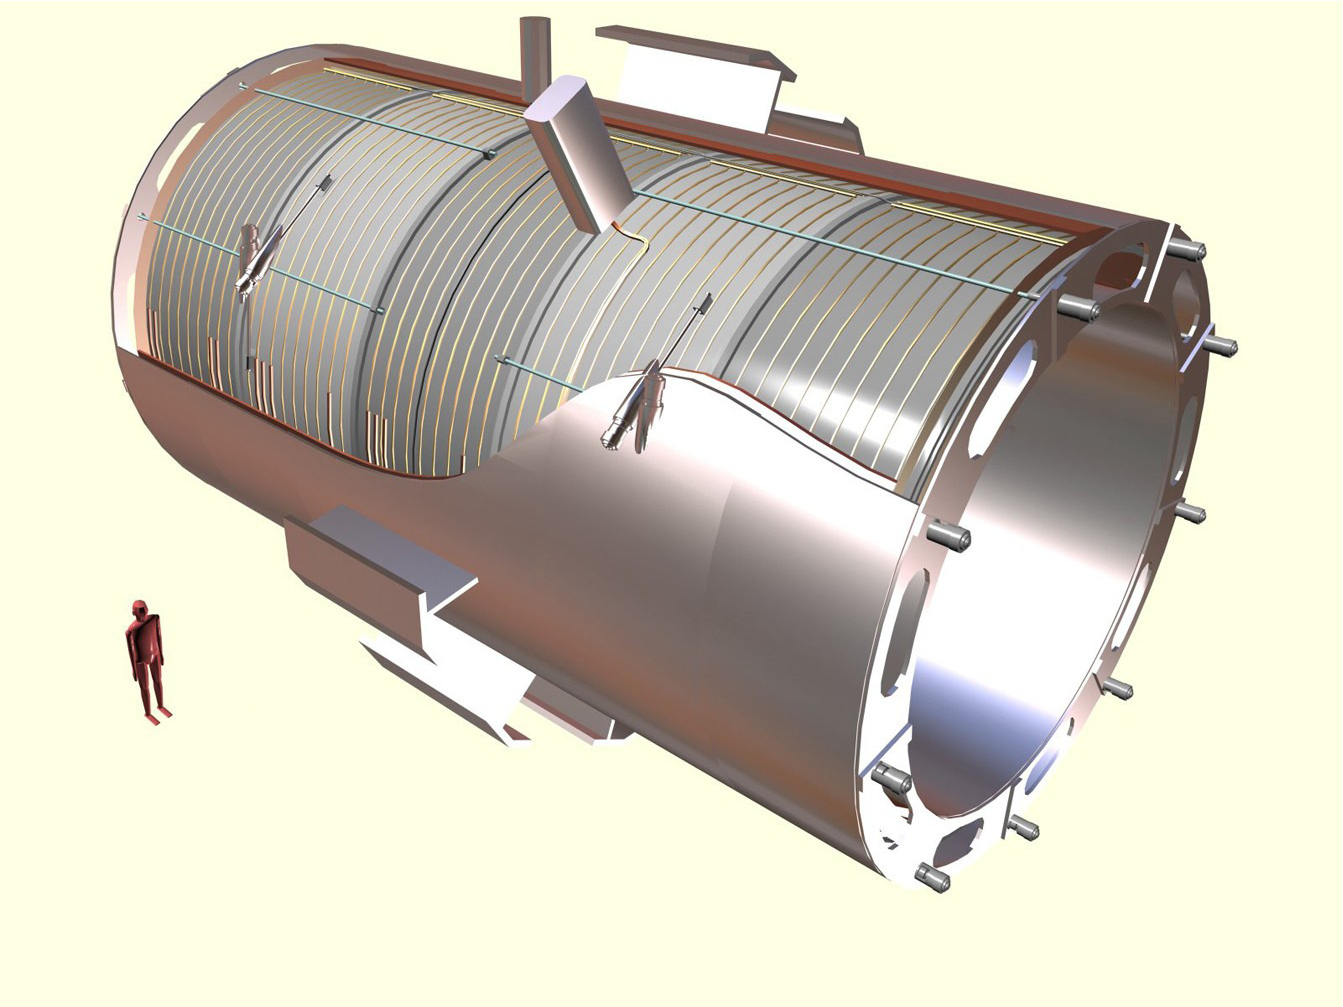
\includegraphics[height=0.2\textheight,clip=true,trim=0 2cm 0 0]{figures/cms/CMS_solenoid}
  ~
  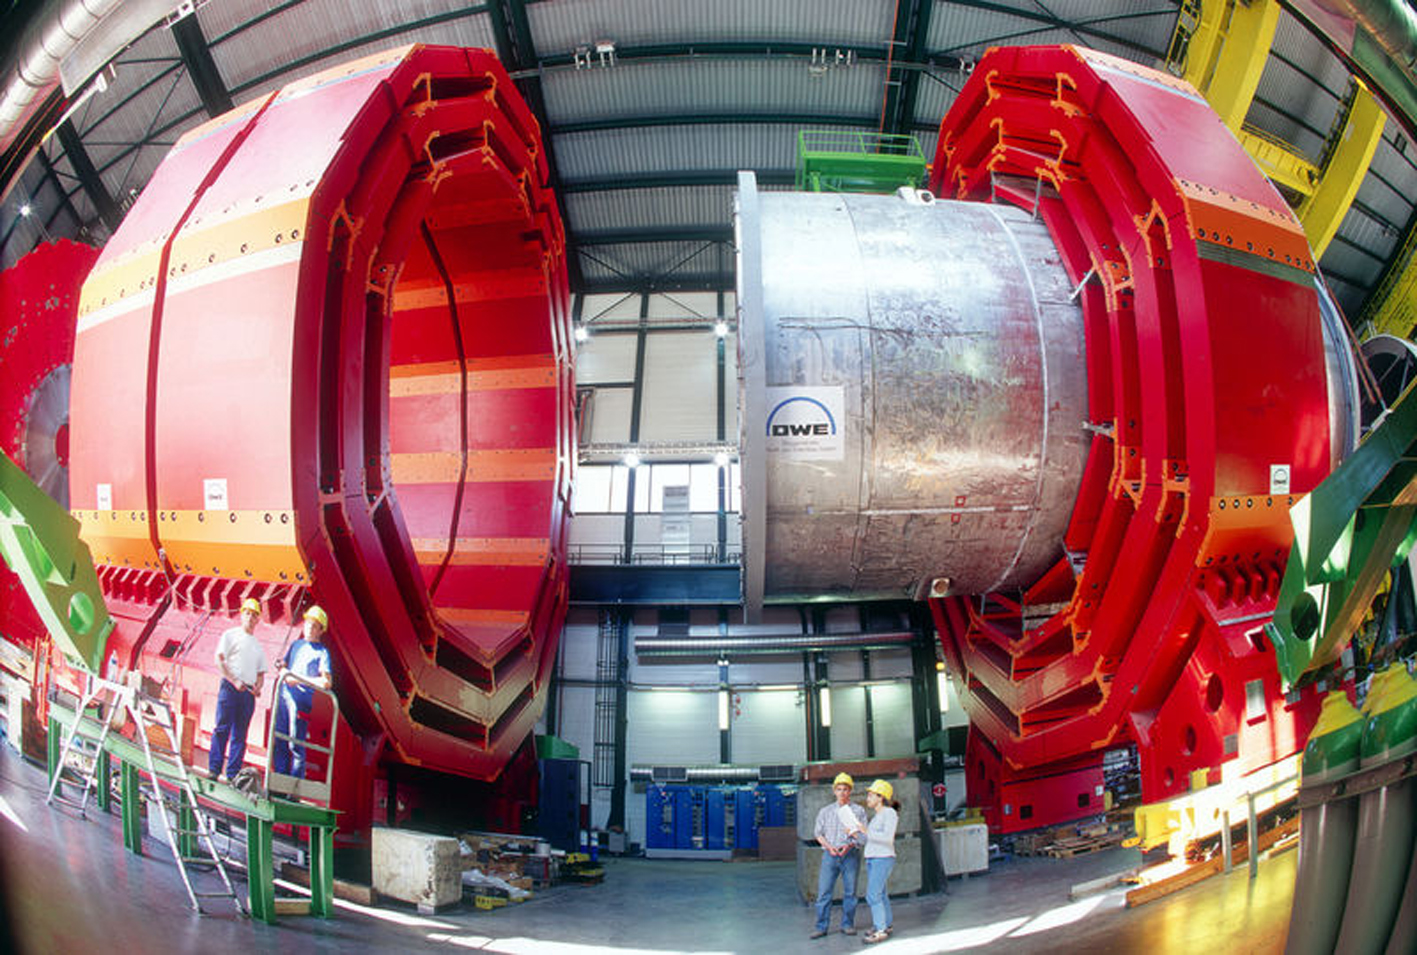
\includegraphics[height=0.2\textheight]{figures/cms/cms_magnet}
  \caption{[left] Artistic view of the superconducting solenoid showing the five modules composing
the cold mass inside the cryostat. Figure taken from Ref.~\cite{Chatrchyan:2008aa}.
  [right] Fish-eye view of the red magnet yoke during construction in
2002. Figure taken from Ref.~\cite{CMS_magnet}.
  \label{fig:cms_magnet}}
\end{figure}

%%%%%%%%%%%%%%%%%%%%%%%%%%%%%%%%%%%%%%%%%%%%%%%%%%%%%%%%%%%%%%%%%%%%%%%%%%%%%%%%%%%%%%%%%%%%%%%%%%%%
\section{Tracker \label{sec:cms_tracker}}

The purpose of the tracker is to very accurately measure the curved tracks of charged
particles with $\pt > 1\GeV$, such that a precise momentum measurement can be made. 
The tracker should also be able to precisely reconstruct secondary
vertices stemming from e.g. $\cPqb$ quark decays. 
In addition, particles should be disturbed the least amount possible while passing through the
tracker. The tracker should thus consist of as little material as possible in order to avoid
multiple scattering, bremsstrahlung, photon conversion, and nuclear interactions.
To accomplish this, the tracker comprises several thin layers. When a particle passes
through a layer, it creates a signal, a \textit{hit}. The reconstruction software then builds a
track out of the different hits. 

The tracker is the innermost layer of the CMS detector, perfectly placed to measure the particles
coming directly from the collision point. Its closeness to the beam pipe also means that it will
receive the largest amount of particles, and thus radiation, which translates into the need for
radiation hard materials. 

The CMS tracker is entirely built out of silicon, and consists of a pixel detector at the very
center, surrounded by a microstrip detector. It has a length of 5.8\meter and a diameter of
2.5\meter. With about 200$\meter^\text{2}$ of active silicon area, the CMS tracker is the largest
silicon tracker ever built. A diagram of the structure is shown in
Fig.~\ref{fig:cms_tracker}, alongside a photograph of part of the strip detector. 
There are a total of 75 million read-out channels with very fast response, providing a precision of
10\mum in position measurement, even when up to 1000 particles traverse the tracker every
25\unit{ns}. This corresponds to a transverse momentum resolution of 1-2\% for $\pt \approx
100\GeV$. 

The pixel detector has three cylindrical layers very close to the collision point (at 4\cm, 7\cm and
11\cm from the beampipe), and two disks at either end. Each of the 65 million pixel sensors measures
100\mum by 150\mum. A cooling system is installed to keep the temperature from rising too much
above the operating temperature of $-10\de$C.

The silicon strip detector consists of ten layers in total. There are four inner barrel (TIB)
layers with two inner endcaps (TID), each composed of three small discs. The outer barrel (TOB)
consists of six layers, while two endcaps (TEC) close off the tracker. The strip tracker is
cooled to a temperature of $-20\de$C in order to minimize the spreading of any radiation
damage.

\begin{figure}[tpb]
  \centering
  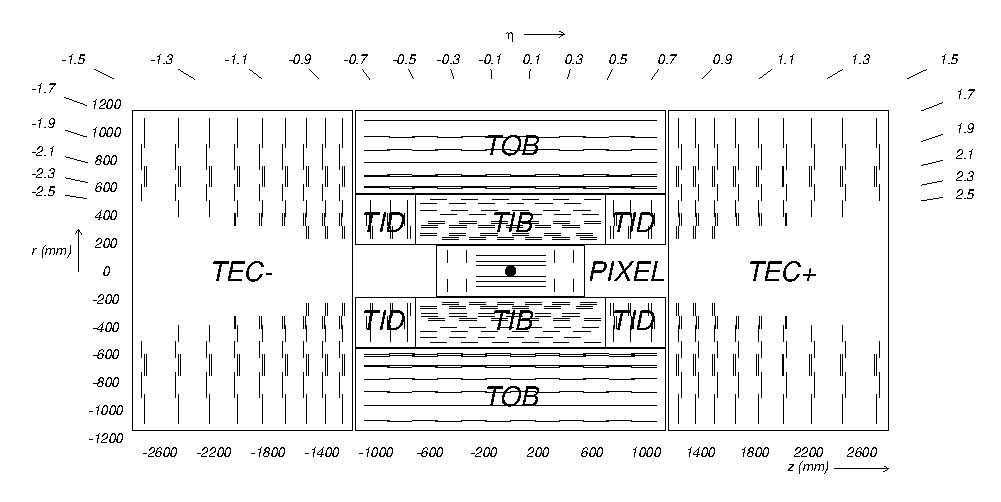
\includegraphics[height=0.17\textheight]{figures/cms/CMS_tracker_general_layout}
  ~
  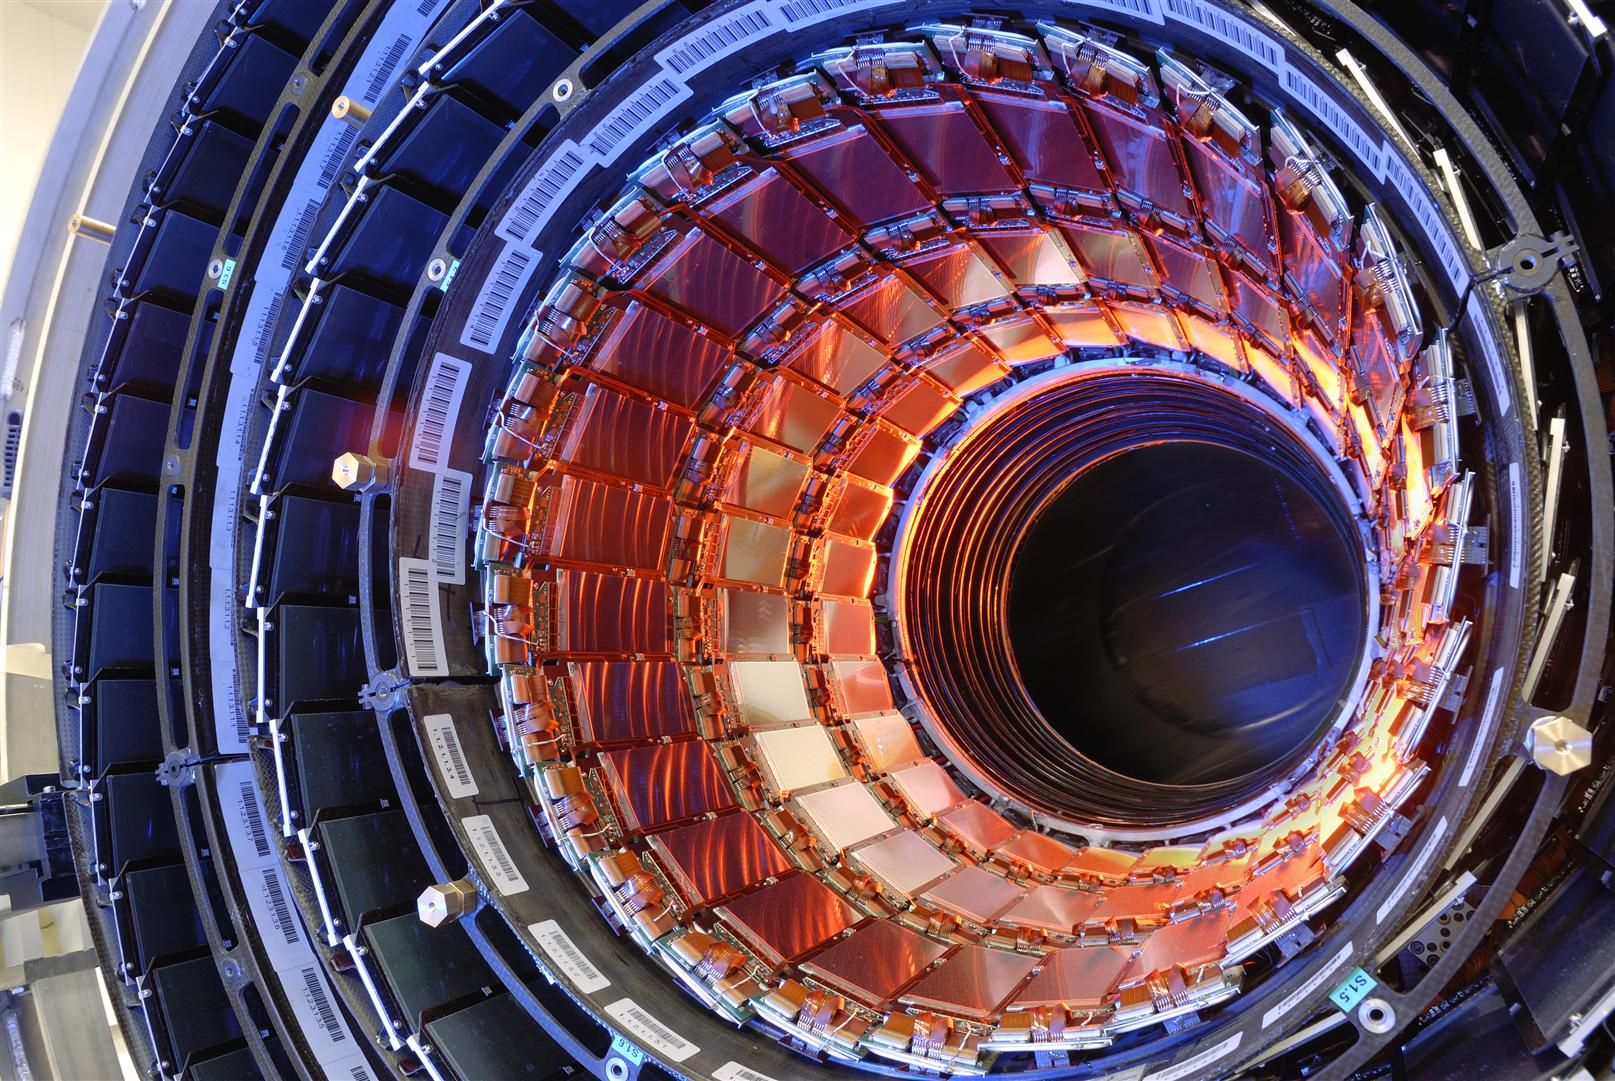
\includegraphics[height=0.17\textheight]{figures/cms/cms_tracker}
  \caption{[left] Schematic cross section through the CMS tracker. Each line represents a detector
module. Figure taken from Ref.~\cite{Chatrchyan:2008aa}. 
  [right] The first half of the CMS inner tracker barrel (TIB), consisting of three
layers of silicon modules. Figure taken from Ref.~\cite{CMS_tracker}.
  \label{fig:cms_tracker}}
\end{figure}

%%%%%%%%%%%%%%%%%%%%%%%%%%%%%%%%%%%%%%%%%%%%%%%%%%%%%%%%%%%%%%%%%%%%%%%%%%%%%%%%%%%%%%%%%%%%%%%%%%%%
\section{Electromagnetic calorimeter \label{sec:cms_ecal}}

The CMS electromagnetic calorimeter is a hermetic homogeneous calorimeter, consisting of a central
barrel region and two endcaps, and is located in between the tracker and the HCAL. 
It has a fine granularity, is fast, and radiation resistant.
The ECAL provides a very good energy resolution for electrons and photons, which played a key role
in the discovery of the Higgs boson in the $h\rightarrow\gamma\gamma$ final state. 

The ECAL is made of about $75\,000$ highly transparent lead tungstate ($\text{PbWO}_\text{4}$)
crystals whose length corresponds to about 25 radiation lengths. A photograph of the crystals
during testing, and a schematic view of the ECAL structure is shown in
Fig.~\ref{fig:cms_ecal_crystal}. The crystals are arranged side-by-side with their longitudinal axes
slightly pointing away from the interaction point to avoid cracks.

When electrons or photons pass through such a lead tungstate crystal, it scintillates. 
This scintillation light is detected, and converted to an electrical signal, by avalanche
photodiodes (APDs) in the barrel, and vacuum phototriodes (VPTs) in the endcaps.
The scintillation decay time is very short, about 80\% of the light is emitted within 25\unit{ns},
which is ideal for the bunch spacing of the LHC. 
The light yield of the crystals depends strongly on temperature, however. In order to keep the
temperature at a stable level, to within 0.1\de C, a dedicated temperature control system was put in
place.
Even though the crystals are quite radiation hard, they still suffer damage in the very high
particle flux environment within CMS. Fortunately, the damage repairs itself through annealing
during the periods when the accelerator is not operational, and the temperature of the crystals is
higher. A light monitoring system is used to accurately measure the transparency of the crystals
throughout the running period, so that precise energy measurements can always be made. 

Preshower detectors in front of the ECAL endcaps provide for extra spatial precision, making it
possible to distinguish between single high-energy photons and the less interesting close pairs of
low-energy photons coming from the decay of neutral pions.
The preshower detector is a sampling calorimeter, consisting of two planes of lead radiators that
initiate showers when an electron of photon passes through. Behind each lead plane are sensors that
measure the deposited energy and transverse shower profiles. 
The sensors are silicon strip detectors of only 2\mm wide, compared to 3\cm for the ECAL endcap
crystals. The two layers of strips are placed orthogonally, thus providing a position
measurement with extremely fine granularity. 


\begin{figure}[htpb]
  \centering
  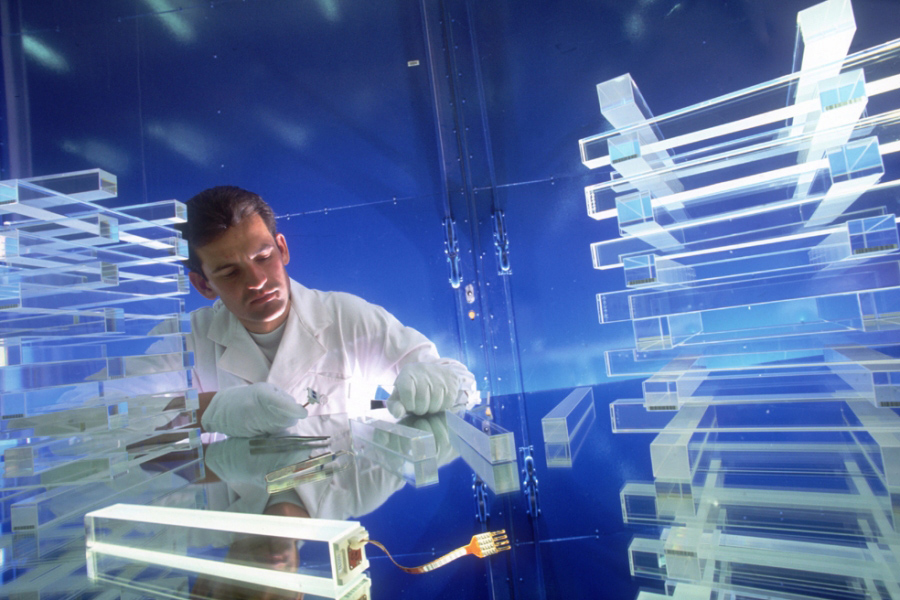
\includegraphics[width=0.48\textwidth]{figures/cms/cms_ecal_crystal}
~
  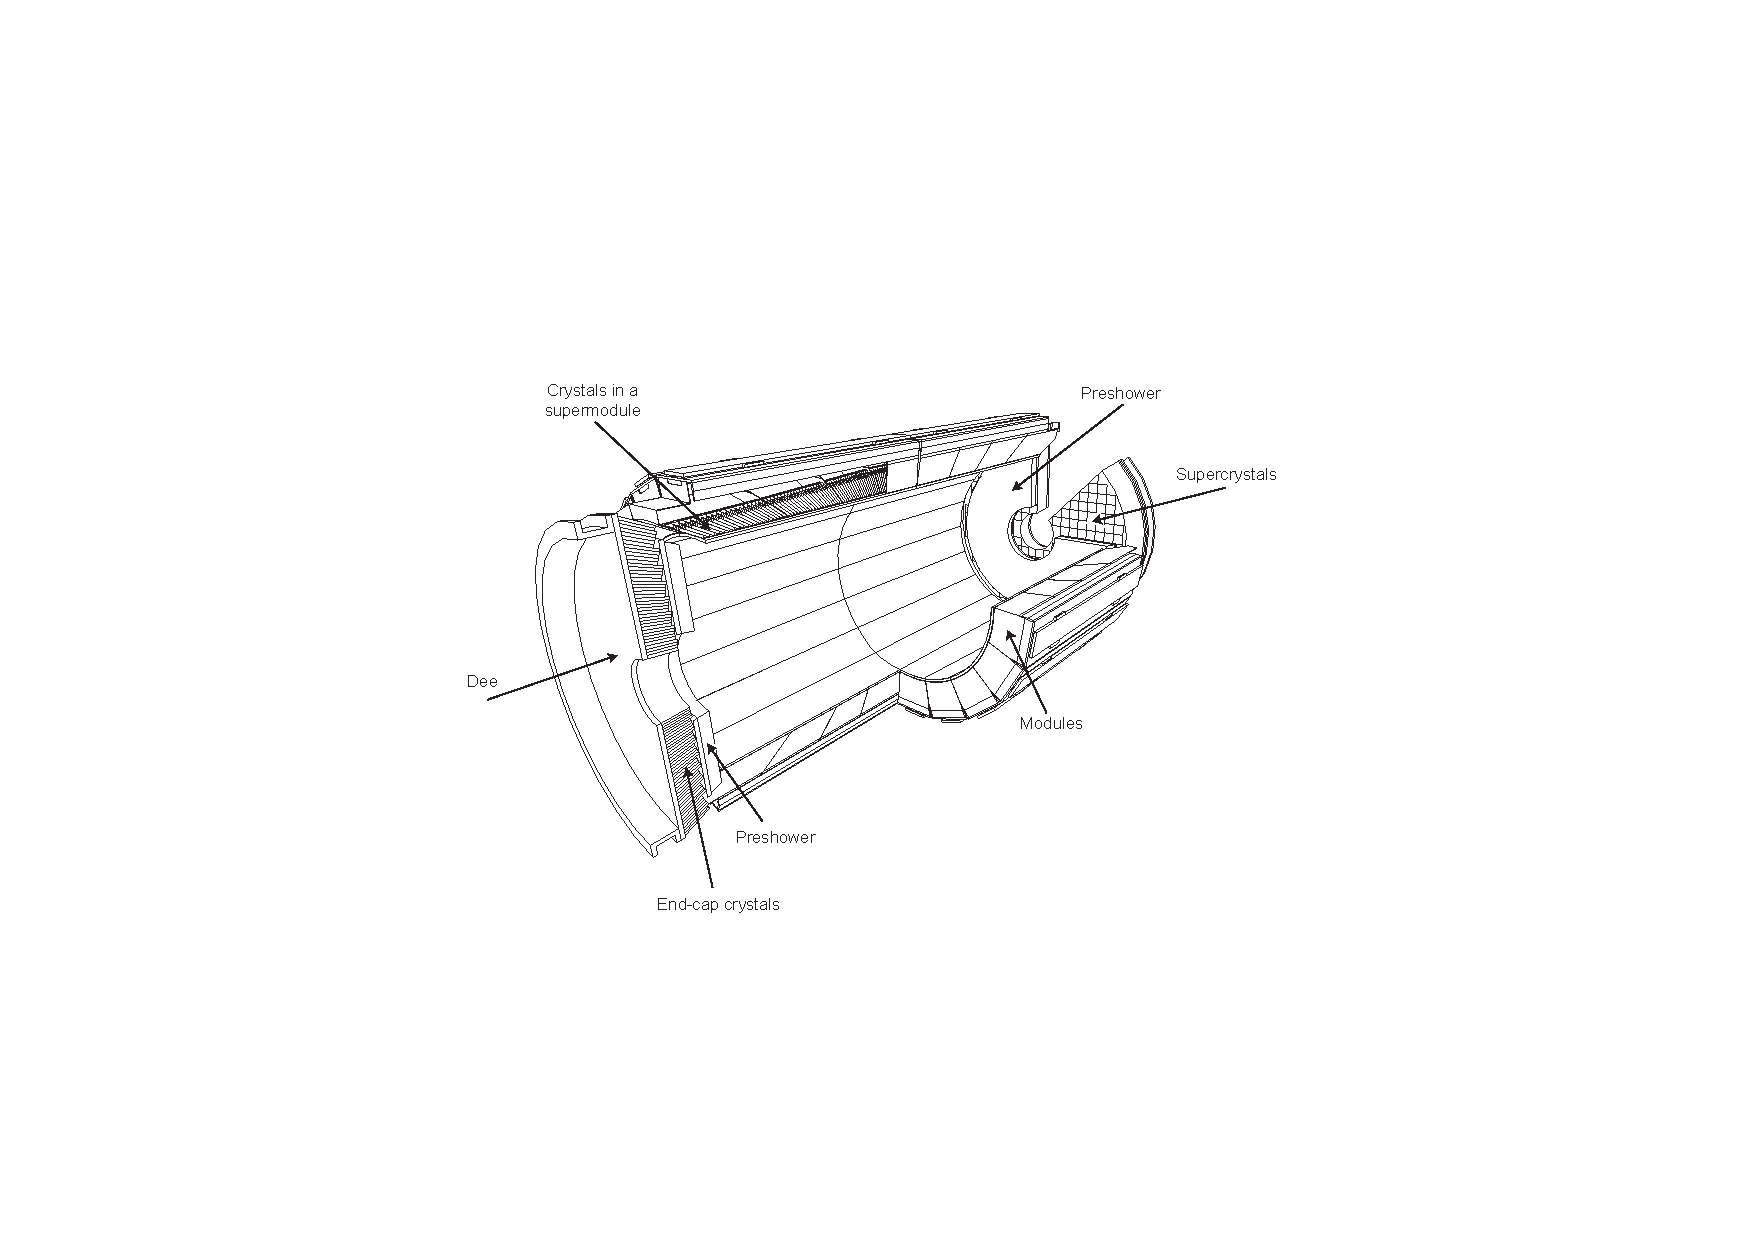
\includegraphics[width=0.48\textwidth]{figures/cms/CMS_ECAL}
  \caption{[left] The construction of the CMS electromagnetic calorimeter: lead-tungstate crystals
being tested in 2005. Figure taken from Ref.~\cite{CMS_ecal_crystal}.
[right] Schematic overview of the ECAL, showing the barrel modules that contain the crystals, the
endcaps, and the preshower detectors. Figure taken from Ref.~\cite{Chatrchyan:2008aa}.
  \label{fig:cms_ecal_crystal}}
\end{figure}

%%%%%%%%%%%%%%%%%%%%%%%%%%%%%%%%%%%%%%%%%%%%%%%%%%%%%%%%%%%%%%%%%%%%%%%%%%%%%%%%%%%%%%%%%%%%%%%%%%%%
\section{Hadron calorimeter \label{sec:cms_hcal}}

The hadron calorimeter is the last subdetector that is (mostly) located within the magnet coil. It
is designed to detect and absorb hadrons, such that the only particles leaving the HCAL are muons
and very weakly interacting particles such as neutrinos.
For this purpose it was built to be as hermetic as possible, staggering the detector layers to
make sure there are no gaps in straight lines that would allow hadrons to escape undetected.
Without this hermeticity it would be impossible to use the missing transverse energy as a way to
infer the presence of very weakly interacting particles. Many new physics searches, e.g. SUSY
searches, would lose most of their sensitivity. 

The HCAL consists of four subparts: the barrel (HB), outer barrel (HO), endcap (HE) and forward
(HF) sections. The barrel and endcap subsystems are sampling calorimeters, made of alternating
layers of dense absorber material (brass or steel) and fluorescent plastic scintillator tiles.
When a hadronic particle hits an absorber plate, an interaction can occur producing numerous
secondary particles. These secondary particles then flow through the successive layers of absorber
material, where they too can interact, resulting in a cascade or “shower” of particles.
As this shower develops, the particles pass through the layers of scintillators, causing them to
emit blue-violet light. This light is absorbed by wavelength-shifting optical fibres, which shift
the light into the green region of the spectrum, before being transported to the readout boxes by
clear optical cables. The amount of light that is collected is a measure of the energy of the
passing particle. Hybrid Photodiodes convert the optical signals into fast electronic signals which
are then sent to the data acquisition system. A photograph of the barrel HCAL is shown on the left
in Fig.~\ref{fig:cms_hcal}. 

To fully absorb a particle shower, about one metre of absorber material is needed. As CMS is a
very compact detector, it was impossible to fit the full HCAL barrel inside the magnet coil. This
is the reason why the outer barrel, the tail-catcher, is located just behind the magnet coil, where
it ensures that the punch-through particles are absorbed as much as possible, rather than create
fake hits in the muon system. 

The two hadronic forward calorimeters are positioned at either end of CMS, at 11.2\meter from
the interaction point, extending the coverage down to very high $|\eta|$. 
The HF receives the bulk of the particle energy contained in the collision, and so must be very
resistant to radiation. The design of the HF was primarily guided by the necessity to survive the
hostile conditions. Over 1000\unit{km} of quartz fibres are inserted into steel absorber
blocks, as can be seen on the right in Fig.~\ref{fig:cms_hcal}. 
When particles traverse these fibres, they generate Cherenkov light. This light is then
transported through the fibers to photomultiplier tubes where it is converted into an electrical
signal. 
The HF is divided into two longitudinal segments, making it possible to distinguish the more shallow
showers generated by electrons and photons, from those generated by hadrons.

\begin{figure}[htpb]
  \centering
  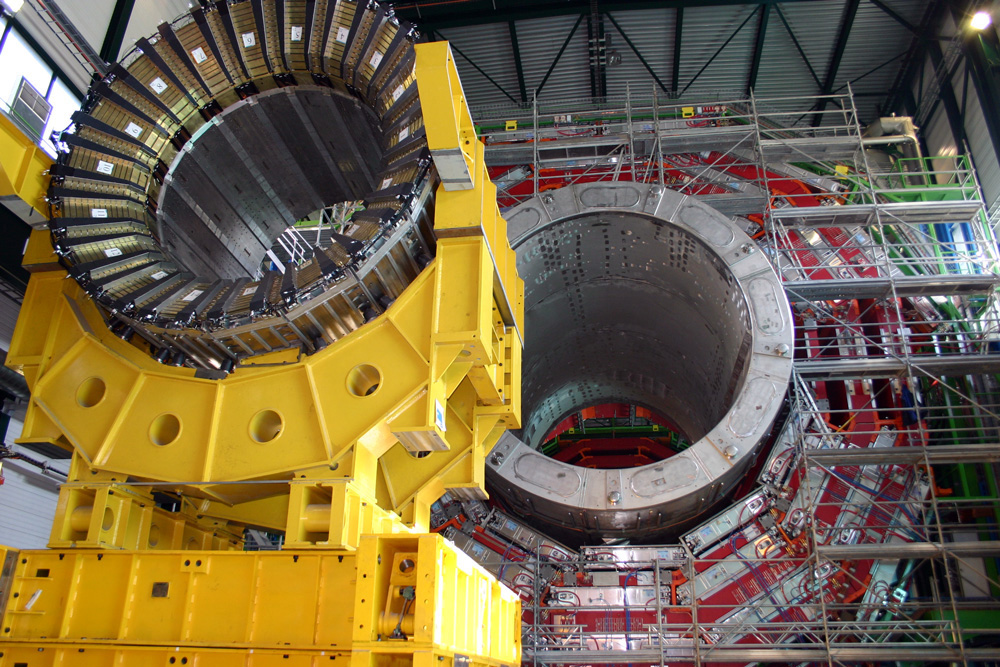
\includegraphics[height=0.2\textheight]{figures/cms/cms_hcal}
~
  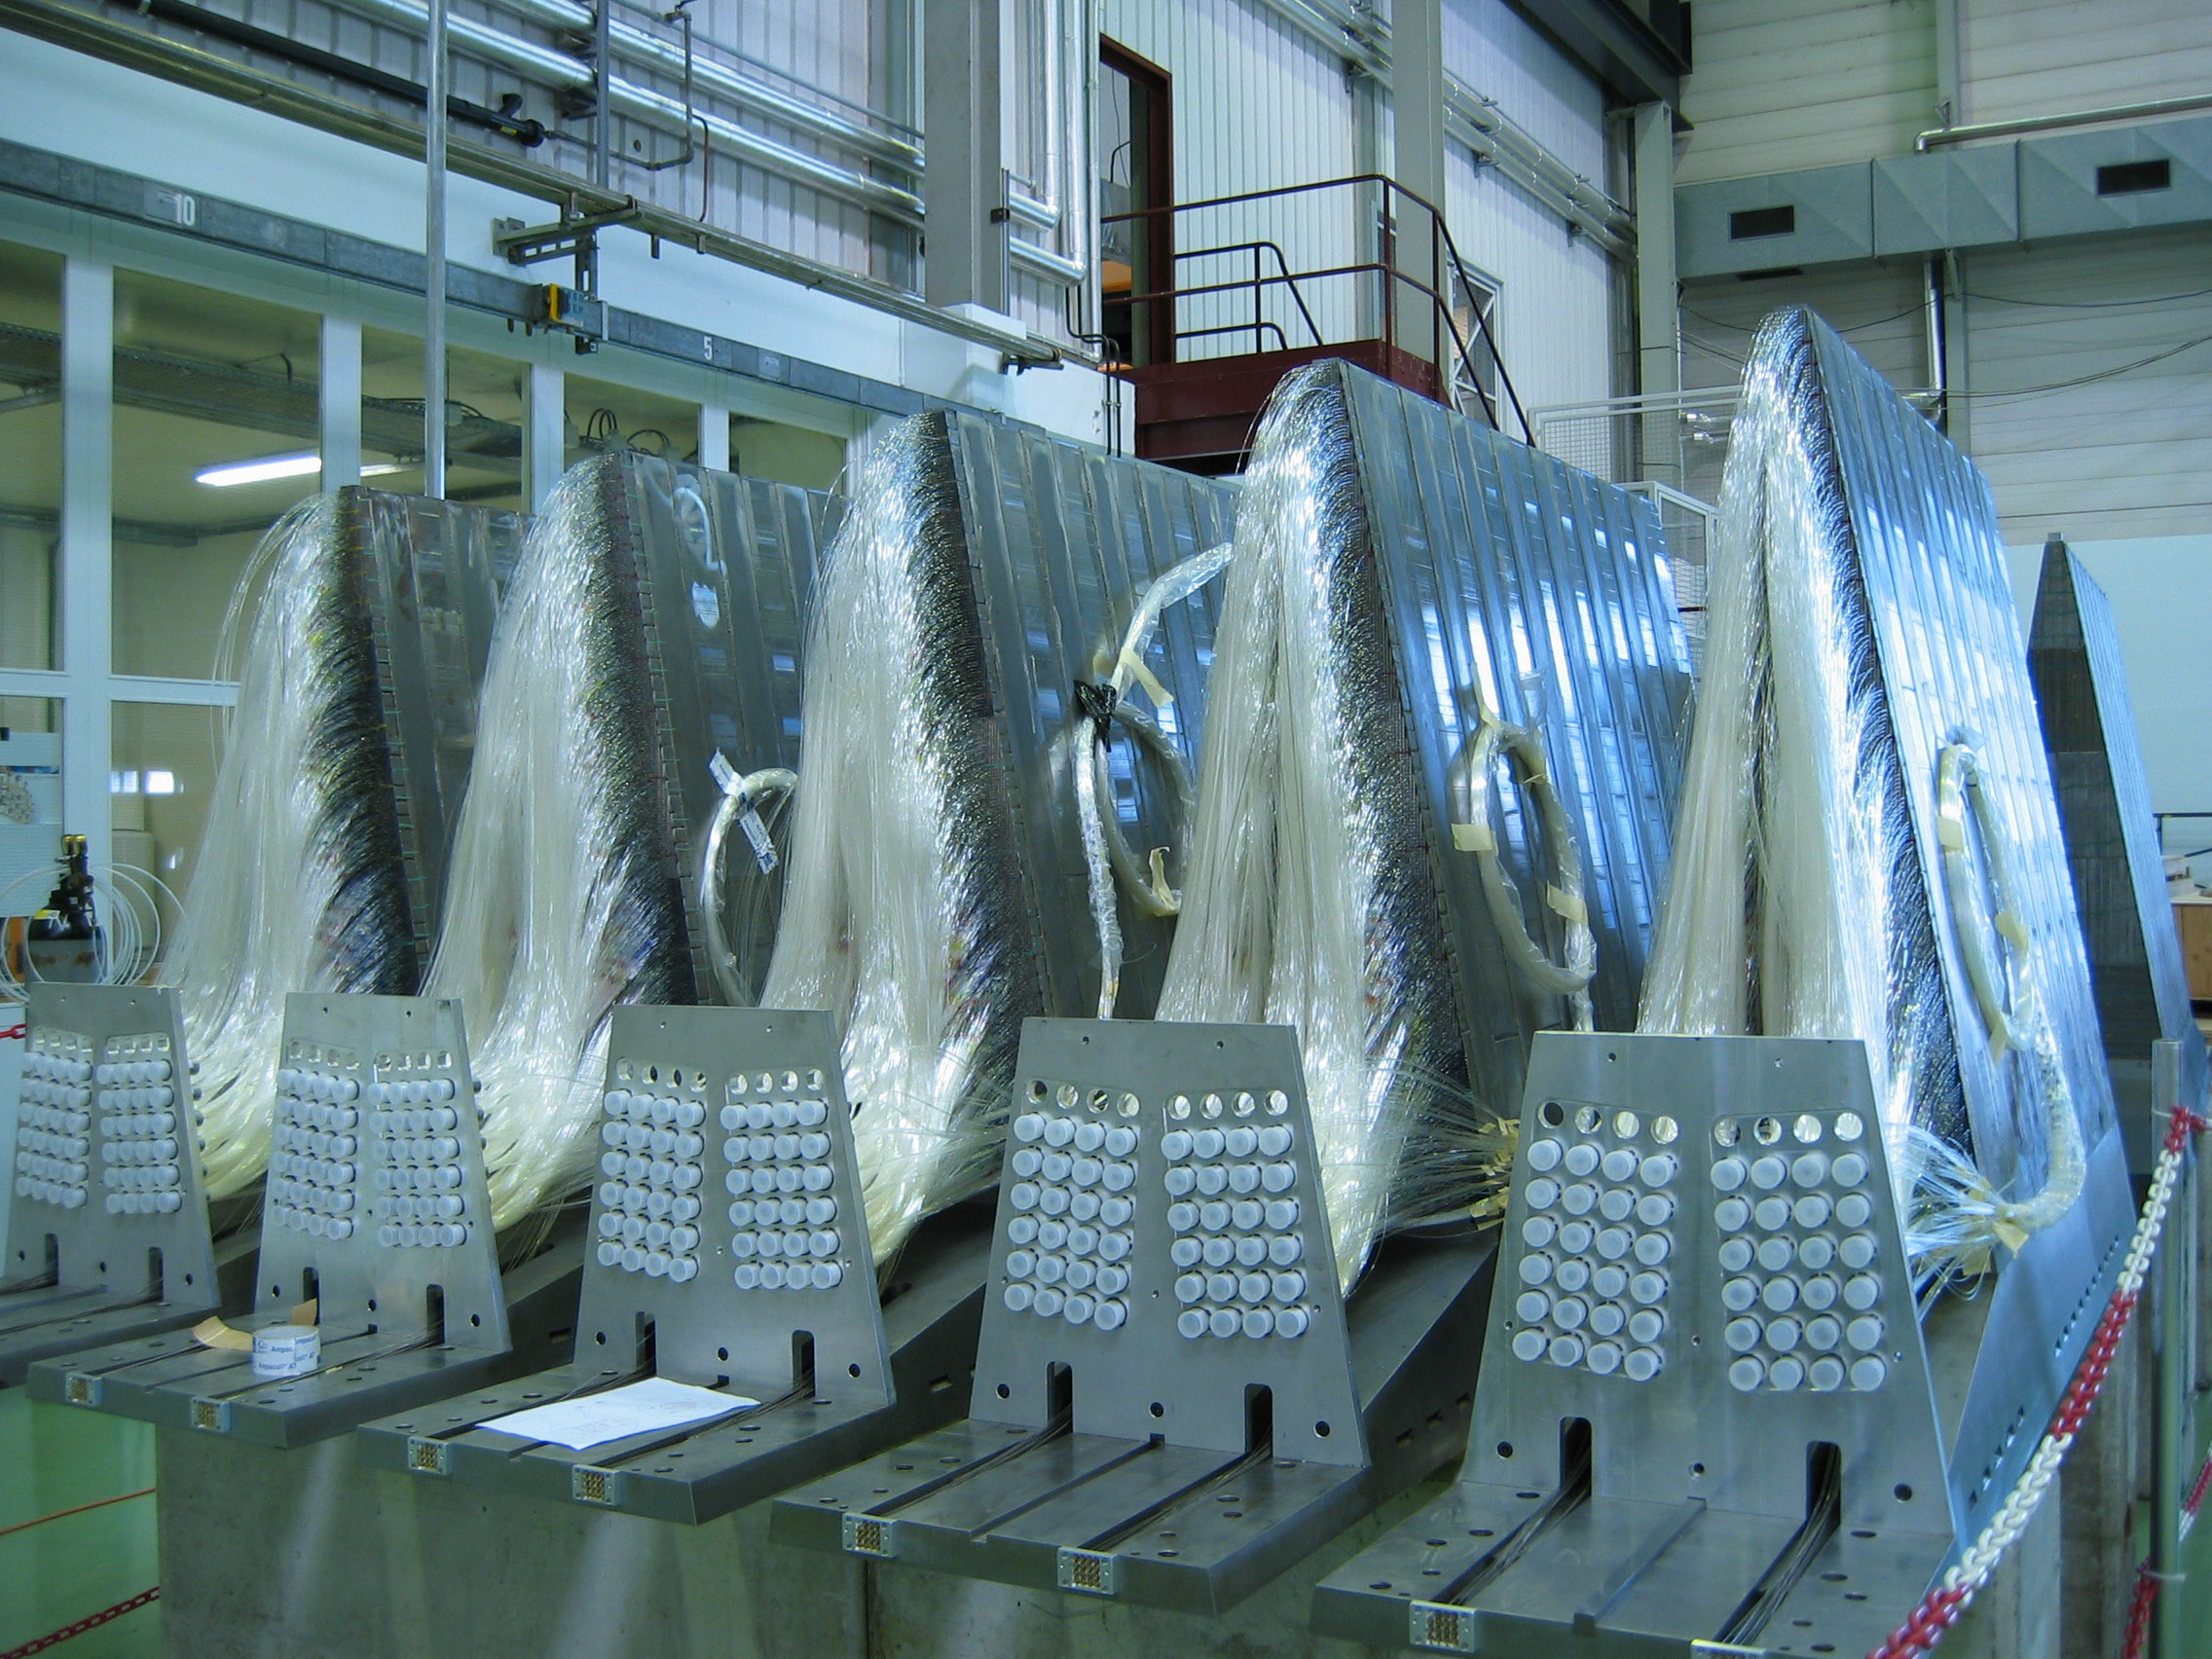
\includegraphics[height=0.2\textheight]{figures/cms/cms_hf_cds1431489}
  \caption{[left] Insertion of part of the barrel HCAL into the solenoid for the Magnet Test
and Cosmic Challenge in 2006. Figure taken from Ref.~\cite{CMS_hcal}.
[right] Segments of the forward HCAL during assembly, showing the quartz fibers inside the steel
wedges. Figure taken from Ref.~\cite{CMS_hf}. 
  \label{fig:cms_hcal}}
\end{figure}

%%%%%%%%%%%%%%%%%%%%%%%%%%%%%%%%%%%%%%%%%%%%%%%%%%%%%%%%%%%%%%%%%%%%%%%%%%%%%%%%%%%%%%%%%%%%%%%%%%%%
\section{Muon system \label{sec:cms_muon_system}}

Detecting muons, the heavier sibling of electrons, is one of the priorities of the Compact
\textit{Muon} Solenoid. Because it is 200 times heavier, a muon interacts less with material than
an electron, enabling it to penetrate several metres of iron, and pass through the calorimeter
systems unstopped. The muon chambers are, therefore, placed behind all the other subdetectors
where muons are the only particles that would register a signal. 
This also means that muons are not easily mistaken for any other particle, thus providing a very
clean signature. The Higgs boson decay to four muons is often referred to as the \textit{golden
channel} for exactly this reason, and it was indeed key to the Higgs boson discovery and the very
accurate measurement of its mass. 

The muon system consists of four muon stations, interleaved with the magnet return yoke, that track
the path of a muon. The momentum of the muon is then inferred from its curvature in the magnetic
field. Three different types of muon chambers are used: resistive plate chambers (RPCs) provide a
very fast trigger decision, while drift tubes (DTs) and cathode strip
chambers (CSCs) provide positional information and additional trigger information.
In the barrel region, DTs and RPCs are arranged in concentric cylinders, whereas the endcap disks
contain different layers of CSCs and RPCs. Figure~\ref{fig:cms_muon_system} shows a schematic view
of the muon system, along with a picture from the barrel muon chambers in the return yoke. 

\begin{figure}[tpb]
  \centering
  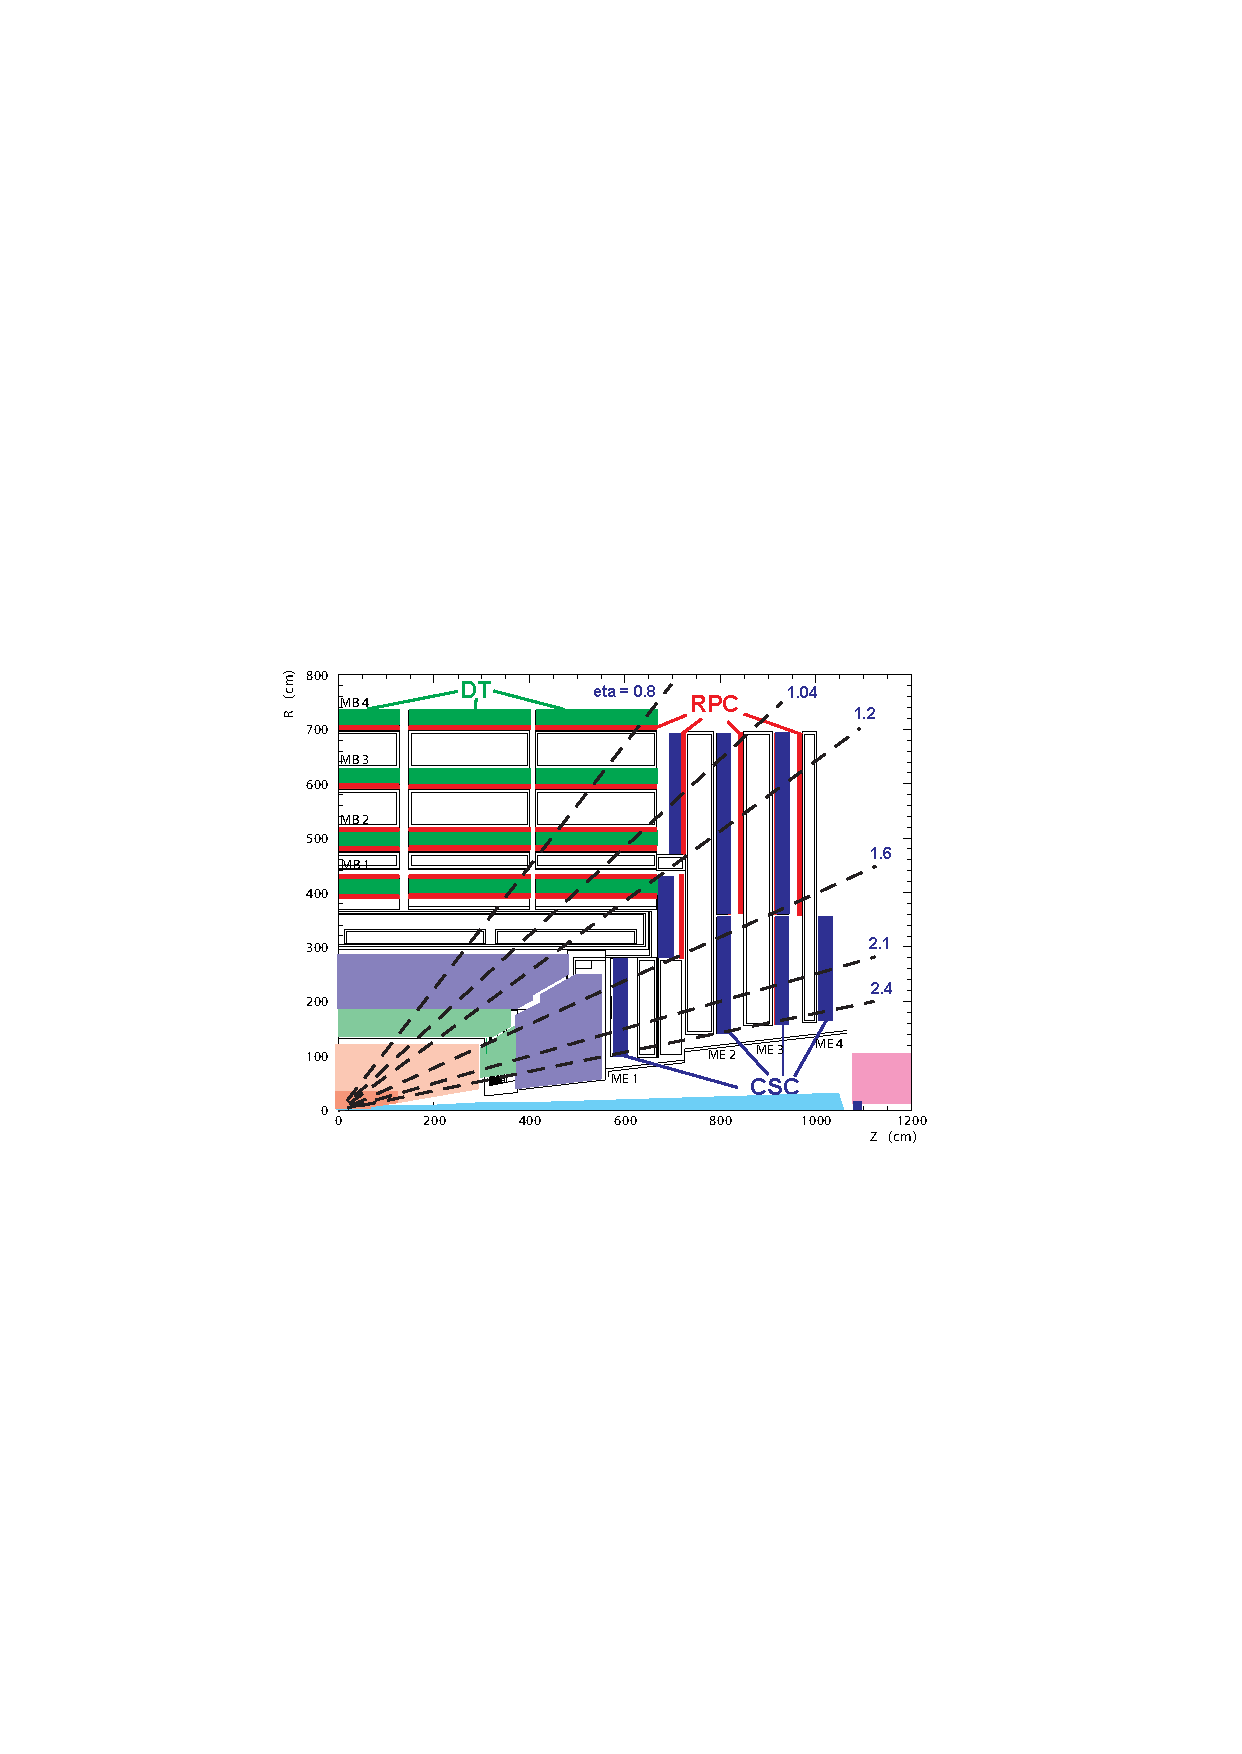
\includegraphics[height=0.205\textheight]{figures/cms/CMS_muon_system_diagram}
~
  \includegraphics[height=0.2\textheight]{figures/cms/cms_muon_system}
  \caption{[left] Schematic overview of one quarter of the CMS muon system, showing the DT, CSC and
RPC detectors. Figure taken from Ref.~\cite{Bayatian:922757}.
  [right] Muon chambers interspersed in the magnet return yoke. Figure taken from
Ref.~\cite{CMS_muon_system}.
  \label{fig:cms_muon_system}}
\end{figure}

\textbf{Drift tubes} contain a stretched wire within a gas volume. Any charged particles passing
through the gas create free electrons, which then drift towards the positively charged wire where
they are registered.  
Each CMS DT chamber, on average 2\meter by 2.5\meter in size, consists of 12 aluminium layers,
arranged in three groups of four, the superlayers, each containing up to sixty 4\cm wide drift
tubes.
The DTs can provide two coordinates for the position of the muon because the superlayers are placed
orthogonally to each other. The $(r, \phi)$ coordinate is measured by wires parallel to the
beampipe, while the $z$ coordinate is obtained from wires perpendicular to the beampipe. 
How far from the wire the muon actually passed, is determined from the electron drift speed and the
arrival time of the electrons at the wire.

\textbf{Cathode strip chambers} are more radiation resistant compared to drift tubes, and are,
therefore, used in the endcap disks where the magnetic field is uneven and particle rates are high. 
The CSCs are so-called multiwire proportional chambers, consisting of positively-charged anode wires
crossed with negatively-charged copper cathode strips inside a gas volume. Muons passing through
one of the 468 trapezoidally shaped CSCs ionize the gas, creating electrons that move
towards the anode wires, and positive ions that move towards the copper cathode. 
Because the strips and the wires are perpendicular, we obtain two position coordinates. The
wires provide the radial coordinate $r$, and the strips the $\phi$ coordinate. 
Given that the wires are very closely spaced, the CSCs are fast and can thus be used as input to the
trigger decision, besides performing the task of precision muon measurement. 

\textbf{Resistive plate chambers} are made of two parallel plates of a very high resistivity
material, a positively-charged anode and a negatively-charged cathode, which are separated by a gas
volume, the \textit{gap}. The CMS RPC system uses 610 double-gap modules comprising two gas gaps
with readout strips in between. 
As for the other muon detectors, passing muons knock electrons out of gas atoms. These electrons
then initiate an avalanche which moves towards the anode. The avalanche is detected by the metallic
readout strips. The pattern of the hit strips gives a measure of the muon momentum. Because RPCs
have a time resolution of just one nanosecond, they are very well suited be part of the muon trigger
system. 



%%%%%%%%%%%%%%%%%%%%%%%%%%%%%%%%%%%%%%%%%%%%%%%%%%%%%%%%%%%%%%%%%%%%%%%%%%%%%%%%%%%%%%%%%%%%%%%%%%%%
\section{Trigger and data acquisition \label{sec:cms_tdaq}}

At design specifications, CMS detects a proton bunch crossing every 25\unit{ns}. This means that
there are 40 million collisions per second, too much to fully read out, process and store for
further analysis. Reducing this amount of data to a more manageable few hundred events
per second is the role of the trigger system. It is of course of prime importance to keep the
interactions that could reveal new phenomena, such as supersymmetry, and discard those that provide
little new information. 
The decision to keep or throw out an event is made in two stages, at the Level-One (L1) Trigger and
the High-Level Trigger (HLT). Both of those systems will be discussed in the next sections. 

The enormous data production rate has another consequence. The collisions occur so fast that the
particles produced in one event have not yet left the detector when the next collision occurs. 
Associating each particle, and thus each detector signal, to the correct bunch crossing is only
possible because of the very good time resolution of the detectors, and the synchronization between
all the readout channels. 
Data from each subdetector is first collected in separate pipelines and is then sent off to the
switch networks to build the full event. Section~\ref{sec:cms_daq} will discuss in more detail how
the events are constructed.

\subsection{L1 Trigger \label{sec:cms_level_one}}

The L1 trigger is designed to make extremely fast decisions, based on relatively simple criteria,
reducing the data rate to about 100\unit{kHz}. 

When particles from a collision pass through the different subdetectors, they generate signals.
These signals are collected in buffers in the front-end electronics of the subdetectors themselves. 
A subset of the information is immediately passed along to the L1 trigger, which is housed
in a service cavern next to the detector. A total time of $3.2\mus$ is allocated for the transit to
the L1 trigger boards, choosing whether to keep or reject the event, and the transit back to the
front-end electronics to execute what was decided. During this time, the total amount of information
on a given collision needs to be kept in the buffers.
Less than 1\mus is allocated to the L1 trigger to perform the calculations needed to make the
decision. It is, therefore, built from custom hardware processors, fully optimized for the task at
hand. 

Because decisions have to be made so quickly, it is impossible to use all available information, so
 only the calorimeters and the muon system are included. 
The trigger objects, such as photons, electrons, muons, and jets, are constructed by the global
calorimeter trigger and global muon trigger, using the reduced granularity and resolution data
sent to them from the front-end electronics. The objects are then passed to the Global Trigger,
which makes the decision to keep an event or not based on the number of objects above given \ET
or \pt thresholds, and/or on the total summed \ET or \ETm of the event. If the event is to be kept,
the high-resolution data is sent from the readout pipelines to the event builder and the High
Level trigger. 

\subsection{High Level Trigger \label{sec:cms_hlt}}

The High Level trigger~\cite{Adam:2005zf} is a computer farm that has access to the full event
information, and can therefore perform complex calculations similar to those made in the offline
analysis software. 
Each event reaching the HLT is sent to a separate processor which spends on average less than
0.1\second to make the final trigger decision, although for some events this can reach up to
1\second. 
The trigger software is set up in such a way that on average only a few hundred events per second
are kept and written to disk. 
A trigger path, a combination of object requirements that specifies which events should
be kept, can be as complex as needed, as long as the computation is fast enough. 
To facilitate this, the trigger paths are set up in such a way that events are discarded as soon as
possible, before reaching the more time consuming parts of the code. 
An example of this could be the use of jets constructed from only calorimeter information, before
adding the information from the numerous tracker readout channels to improve precision. 
Each event that is kept receives a set of tags associated with the separate trigger paths that were
fulfilled. These tags are later used to sort the data into so-called primary datasets. 


% HLT refs \cite{Adam:2005zf,Agostino:2009nva}

\subsection{Data acquisition \label{sec:cms_daq}}

The CMS data acquisition (DAQ) system~\cite{Cittolin:578006} comprises different components, which
are illustrated in Fig.~\ref{fig:cms_event_builder}. 
The about 700 detector front-end drivers store the data from the detector front-end electronics upon
the reception of an accept signal from the L1 Trigger. The data are then read by the readout system
and stored until they are sent to the HLT for further processing. 
The builder network provides the interconnections between the readout and the HLT systems, running
with a bandwidth of 100\unit{GB/s}. It takes care of building the full events out of the different
data fragments from the separate parts of the detector. The builder networks consists of 500 builder
units, each of which will assemble the data for one event. 
Once the event is assembled it is passed to one of the HLT processors associated to that particular
builder unit. As soon as the HLT decision is made, that decision is transferred back to the builder
unit which then either discards the event, freeing up memory, or sends it to the storage
manager to be written to disk.
Apart from building the events, the DAQ also provides detector control and monitoring services.

\begin{figure}[htpb]
  \centering
  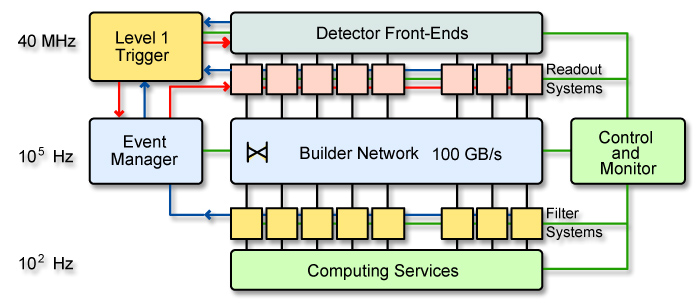
\includegraphics[width=0.8\textwidth]{figures/cms/cms_event_builder}
  \caption{ General architecture of the CMS DAQ System. Figure taken from
Ref.~\cite{Bayatian:922757}.
  \label{fig:cms_event_builder}}
\end{figure}


% refer to next chapter for event reconstruction